\documentclass[a4paper,11pt,french]{book}
\usepackage[utf8]{inputenc}

\usepackage[T1]{fontenc}
\usepackage[francais]{babel} 
\usepackage[top=2cm, bottom=2cm, left=2cm, right=2cm, includeheadfoot]{geometry} %pour les marges
\usepackage{lmodern}
\usepackage{pict2e}
\usepackage{tikz}	
%\usepackage{tikz-uml}
\usepackage{fancyhdr} % Required for custom headers
\usepackage{lastpage} % Required to determine the last page for the footer
\usepackage{extramarks} % Required for headers and footers
\usepackage{graphicx} % Required to insert images
\usepackage{tabularx, longtable}
\usepackage{color, colortbl}
\usepackage{lscape}
\usepackage[hidelinks]{hyperref}
\usepackage{longtable}
\usepackage{multirow}
\usepackage{rotating}
\usepackage{pgfgantt}
\usepackage{gensymb}
\usepackage[toc,page]{appendix} 
\usepackage{pgfplots}
\usepackage{eurosym}
\usepackage{rotating}
\usepackage{array}
\usepgflibrary{arrows} % for pgf-umlsd

\usetikzlibrary{trees,shapes.geometric,arrows,decorations.pathmorphing,backgrounds,fit,positioning,shapes.symbols,chains	}
 \tikzset{
    %Define standard arrow tip
    >=stealth',
    %Define style for boxes
    punkt/.style={
           rectangle, dashed,
           rounded corners,
           draw=black, very thin,
           minimum height=2em,
           minimum width = 2cm,
           text centered},
    square/.style={
           rectangle,
           draw=black, thick,
           minimum height=.5cm,
           minimum width = 1cm,
           text centered},
    data/.style={
           rectangle,
           draw=black, thick,
           minimum height= 2cm,
           minimum width = 2cm,
           text centered},
    % Define arrow style
    pil/.style={
           ->,
           thick,
           shorten <=1pt,
           shorten >=1pt,},
    asym/.style={
           <->,
           thin,
           shorten <=1pt,
           shorten >=1pt,
           red!100},
    sym/.style={
           <->,
           thin,
           shorten <=1pt,
           shorten >=1pt,
           blue!100}
}


%\usetikzlibrary{trees,shapes.geometric,arrows,decorations.pathmorphing,backgrounds,fit,positioning,shapes.symbols,chains	}

\linespread{1.1} % Line spacing

% Set up the header and footer
\pagestyle{fancy}
\lhead{\textbf{\hmwkClass -- \hmwkSubject \\ \hmwkTitle \\ \hmwkDocName}} % Top left header
\rhead{
\includegraphics[width=10em]{logo_univ.png}}
\lfoot{\lastxmark} % Bottom left footer
\cfoot{} % Bottom center footer
\rfoot{Page\ \thepage\ } % Bottom right footer
\renewcommand\headrulewidth{0.4pt} % Size of the header rule
\renewcommand\footrulewidth{0.4pt} % Size of the footer rule

\setlength{\headheight}{40pt}

\newcommand{\hmwkTitle}{Chat sécurisé} % Assignment title
\newcommand{\hmwkClass}{Master 1 SSI } % Course/class
\newcommand{\hmwkAuthorName}{Charles Ango, Ismael Kabore,  Julien Legras, Yves Nouafo, Jean-Baptiste Souchal} % Your name
\newcommand{\hmwkSubject}{Conduite de projet} % Subject
\newcommand{\hmwkDocName}{Rapport de projet} % Document name

\newcommand{\version}{1.2} % Document version
\newcommand{\docDate}{24 mai 2013} % Document date
\newcommand{\checked}{Magali Bardet} % Checker name
\newcommand{\approved}{} % Approver name

\definecolor{gris}{rgb}{0.95, 0.95, 0.95}

\title{
\vspace{2in}
\textmd{\textbf{\hmwkClass :\ \hmwkTitle}}\\
\normalsize\vspace{0.1in}\small{Due\ on\ \hmwkDueDate}\\
\vspace{0.1in}\large{\textit{\hmwkClassInstructor\ \hmwkClassTime}}
\vspace{3in}
}

\author{\hmwkAuthorName}
\date{} % Insert date here if you want it to appear below your name

\makeatletter
\def\chapter{\if@openright\cleardoublepage\else\clearpage\fi
  \global\@topnum\z@
  \@afterindentfalse
  \secdef\@chapter\@schapter}
\makeatother


\begin{document}
\pagestyle{empty}

\vspace*{1cm}
\begin{center}

\includegraphics[width=20em]{logo_univ.png}
\end{center}
\vspace*{2cm}
\begin{center}\textbf{\huge{Master 1 Sécurité des systèmes informatiques}}\end{center}
\vspace*{1cm}
\begin{center}
\textbf{\Huge{\hmwkDocName}: \hmwkTitle}
\end{center}

\vspace*{3cm}
	

\fcolorbox{black}{gris}{
\begin{minipage}{15cm}
\begin{tabularx}{10cm}{lXp{8cm}}
	& & \\
	\bfseries{Rédigé par} & & \hmwkAuthorName \\
	& & \\
	\bfseries{À l'attention de} & & \checked \\
	& & \\
	\bfseries{Date de rendu} & & \docDate\\
	& & \\
\end{tabularx}
\end{minipage}
}

\newpage


%%%%%%%%%%%%%%%%%%%%%%%%%%%%%%%%%%%%%%%%%%%%
% Introduction
% JB
%%%%%%%%%%%%%%%%%%%%%%%%%%%%%%%%%%%%%%%%%%%%
\frontmatter
\pagestyle{fancy}
\large
\chapter{Introduction}


%La table des matières
\tableofcontents



\newpage
\mainmatter
%%%%%%%%%%%%%%%%%%%%%%%%%%%%%%%%%%%%%%%%%%%%
% PRÉSENTATION DU PROJET 
% Yves & Julien
%%%%%%%%%%%%%%%%%%%%%%%%%%%%%%%%%%%%%%%%%%%%
\chapter{Présentation du projet}
Dans le cadre de notre projet, il nous à été demandé de réaliser un chat sécurisé. Pour le mener à bien, le travail à été découpé en deux grandes phases qui sont l'analyse des besoins du client et les solutions proposées.

\section{Besoins du client}
Les besoins du logiciel sont les points indispensables, nécessaires et imposés par le client. Ce sont ces exigences qui détermineront les fonctionnalités du logiciel. Les exigences sont les suivantes:
\vspace{.5cm}
\begin{itemize}\item gestion de la création et de la suppression d’un compte utilisateur;\item création par un utilisateur d’une salle de discussion privée;\item ajout et suppression d’un utilisateur autorisé dans une salle privée;\item confidentialité, intégrité et authentification sur les messages échangés;\item non répudiation des messages;\item création d’une autorité de certification;\item demande de certificat pour l’accès à un salon privé et la communication sécurisée.\end{itemize}

\section{Solutions proposées}
\`A l'issue de l'analyse des besoins du client, il a été convenu de traiter la demande du client en décomposant la réalisation du logiciel en trois phases de développement qui sont:
\begin{enumerate}\item la mise en place du système de bavardage;\item l'installation d'une PKI (infrastructure de clés publiques);\item la mise en place d'une couche sécurisée pour permettre une communication chiffrée.\end{enumerate}
\vspace{.5cm}

\subsection{Structure du logiciel}
Le logiciel est conçu et pensé de manière modulable de tel sorte que chaque partie puisse \^etre utilisée de manière indépendante. L'architecture du logiciel est la suivante:\\

\begin{tikzpicture}[node distance=-.01cm,font=\tiny,scale=1.8,every node/.style={transform shape}]
		\node[square, text width=1cm, fill=white!100] (appclient) at (0,0) {Application client};
		\node[square, text width=1.5cm, fill=white!100] (modclientsec) at (2.5,0) {Module client sécurisé};
		\begin{pgfonlayer}{background} 
		\node[punkt, fit=(appclient)(modclientsec), fill=blue!20] (groupclient) {};
		\end{pgfonlayer}
		
		\node[square, text width=1cm, fill=white!100] (PKI) at (1.4,-1.5) {PKI};
		\node[square, text width=1cm, fill=white!100] (serveur) at (0,-2.5) {Serveur};
		\node[square, text width=1.5cm, fill=white!100] (serveurs) at (2.5,-2.5) {Serveur sécurisé};
		\begin{pgfonlayer}{background} 
		\node[punkt, fit=(PKI)(serveur)(serveurs), fill=green!20] (groupserveur) {};
		\end{pgfonlayer}

		\node[text width=.7cm] (imgbd1) at (0,-4) {
\includegraphics[height=3em]{computer-database.png}};
		\node[square, text width=.5cm, below=of imgbd1, fill=white!100] (bd1){BDD};
		\node[text width=.7cm] (imgfichiers) at (1.4,-4) {
\includegraphics[height=3em]{computer-database.png}};
		\node[square, text width=.7cm, below=of imgfichiers, fill=white!100] (fichiers){BDD};
		\node[text width=.7cm] (imgbd2) at (2.8,-4) {
\includegraphics[height=3em]{computer-database.png}};
		\node[square, text width=.5cm, below=of imgbd2, fill=white!100] (bd2){BDD};

		\begin{pgfonlayer}{background} 
		\node[punkt, fit=(imgbd1) (bd1) (imgbd2) (bd2) (imgfichiers) (fichiers), fill=orange!20] (stock) {};
		\end{pgfonlayer}


		\draw (appclient.east) edge[<->] (modclientsec.west);
		\draw (appclient.south) edge[<->] (serveur.north);
		\draw (modclientsec.south west) edge[<->] (PKI.north);
		\draw (modclientsec.south) edge[<->] (serveurs.north);
		
		\draw (serveur.south) edge[<->] (imgbd1.north);
		\draw (serveurs.south) edge[<->] (imgbd2.north);
		\draw (PKI.south) edge[<->] (imgfichiers.north);
		\draw (PKI.south east) edge[<->] (serveurs.north);
		
		\draw (PKI.west) edge[->, loop left = 90] (PKI.west);

		\end{tikzpicture} \\\vspace{.3cm}
		
La partie 1 met en place le coté client de l'application. Elle est constituée de deux grandes parties qui sont l'application cliente et le module client sécurisé. L'application cliente permettra de réaliser toute la partie communication non sécurisé dont les principales fonctionnalités sont décrites ci-dessous.
\begin{itemize}\item création d’un compte sécurisé; \item envoi de message sur salon privé; \item envoi de message sur salon général;\item rejoindre un serveur de chat sans authentification;\item quitter un serveur de chat;\item envoi d’un message privé non sécurisé;\item créer un salon privé; \item joindre un salon privé; \item fermeture d’un salon privé.\end{itemize}
\vspace{.12cm}
Quant à la partie module client sécurisé, elle permettra d'établir une communication sécurisée dont les fonctionnalités seront décrites dans la partie relative à la mise en place de sécurité. La partie 1 est la partie applicative de l'application.\\

La partie 2 permet de mettre en place une pki (infrastructure de clés publiques). Cette infrastructure permettra de délivrer les clés nécessaire pour la communication entre les utilisateurs connectés, mais aussi de d'authentifier des utilisateurs présent sur le système de bavardage. Nous avons opté pour une pki déjà existante EJBCA qui remplira les fonctionnalités suivantes.
\begin{itemize}\item ajout certificat à un utilisateur;\item révocation d’un certificat;\item renouvellement des clefs des salons privés.\end{itemize}
Dans cette partie, on retrouve les serveurs sécurisés et non sécurisés qui ont pour respectivement pour rôle de permettre la communication entre deux clients et délivrer les clefs symétriques aux utilisateurs pour pouvoir établir une communication privée entre deux utilisateurs sécurisés. L'ensemble de ces trois éléments constitue la partie réseaux de l'application.\\

La partie 3 décrit les bases de données utilent à l'application. Ces bases sont au nombres de trois.\\
Le premier permet la gestion des utilisateurs non sécurisés. Cette gestion se fait via le serveur non sécurisé. Les utilisateurs seront gérés par une base de donnée temporaire (liste chainée) pour déterminer l'existance d'un utilisateur déjà présent.\\ 
Le second permet le stockage des certificats générés par la PKI. Ces certifcats seront stockés dans une base de données interne à l'application EJBCA.\\ 
La dernière base de données permet le stockage des utilisateurs sécurisés qui se fera via le serveur sécurisé dans une base de données embarquée où seront répertoriés les pseudonymes des utilisateurs et le champ "subject" correspondant au certificat qui leur sera attribué.

\subsection{Détail de la couche sécurisée}
La couche sécurisée est nécessaire pour echanger des messages sécurisés sans que celui-ci ne puisse être lu par un autre utilisateur. Dans cette partie, l'utilisation de la bibliothèque OpenSSL a été choisie pour assurer la mise en place d'un canal de communication sécurisé entre deux utilisateurs sécurisés.\\La PKI et le serveur sécurisé intervienent dans la couche sécurisée car la PKI permet de délivrer des certificats aux utilisateurs sécurisés et le serveur sécurisé permet de délivrer les clefs de communication nécessaire entre deux utilisateurs sécurisés. Pour garantir que l'application fourni respecte bien les exigences du client, l'application réalise les exigences fonctionnelles suivantes:
\begin{itemize}\item création d’un compte sécurisé;\item suppression compte sécurisé par l’utilisateur sécurisé;\item rejoindre un serveur de chat sécurisé avec authentification; \item quitter un serveur de chat sécurisé;\item exclure utilisateur sécurisé d’un salon privé;\item invitation d’un utilisateur sécurisé dans un salon privé;\item envoi d’un message privé sécurisé.\end{itemize}
\vspace{.6cm}
Il est à souligner que toutes les fonctionnalités réalisées par un utilisateur non sécurisé peuvent \^etre réalisées par un utilisateur sécurisé.\\

\subsection{choix des langages}
.\\
Le choix des langages pour réaliser le projet sont le C pour la réalisation du serveur non sécurisé et du serveur sécurisé ainsi que des client, sécurisé et non sécurisés.\\La réalisation de la base de données embarquée s'est faite en sqlite.\\La partie graphique quant à été faite en Vala, car ce langag s'exporte en C très facilement.\\
Pour la partie sécurisé on a choisi la bibliothèque OpensSSL pour les raisons vues ci-dessus.

\section{Résultat}

Le résultat a été réparti en trois livraisons dont voici les contenus.

\subsection{Partie non-sécurisée}
La première partie consistait en le développement d'un client et d'un serveur de chat. Dans cette partie, les fonctionnalités ayant été développées sont :
\begin{itemize}
\item se connecter à un serveur de chat;
\item créer, rejoindre et quitter un salon de chat;
\item envoyer des messages privés aux utilisateurs connectés sur le serveur;
\item se déconnecter d'un serveur de chat.
\end{itemize}

Pour la communication entre les clients et le serveur, une structure C a été mise en place :

\begin{verbatim}
typedef struct {
        int code;
        char sender[MAX_NAME_SIZE];         // MAX_NAME_SIZE = 64
        char content[MAX_MESS_SIZE];        // MAX_MESS_SIZE = 512
        char receiver[MAX_ROOM_NAME_SIZE];  // MAX_ROOM_NAME_SIZE = 64
} message;
\end{verbatim}

Chaque action est représentée par un code (\verb+CONNECT, CREATE_ROOM, MESSAGE...+). Le champ \verb+sender+ représente l'émetteur du message, \verb+receiver+ le destinataire. Enfin le champ \verb+content+ contient le(s) argument(s) associé(s) à l'action souhaitée. Côté client, pour envoyer une telle structure, il suffit d'appeler la fonction \verb+int send_message(const char *mess,+\\ \verb+char **error_mess)+ avec \verb+mess+ de la forme : \verb+"/<ACTION> <ARGS>"+ et \verb+err_mess+ le message d'erreur, si une erreur survient. L'affichage de message reçu se fait à la couche supérieur, dans l'interface graphique ou en lignes de commandes en appelant la fonction \verb+int receive_message(+\\\verb+message *m)+. Ces fonctions se trouvent dans une librairie écrite pour le client (\verb+libclient.a+) afin de les utiliser dans l'interface graphique et en préparation à la surcouche sécurisée de la troisième livraison. 

L'interface du client de chat a été développée en Vala à l'aide de la bibliothèque graphique GTK. La fenêtre a été dessinée à l'aide de Glade qui est un User Interface Designer produisant un fichier \verb+.xml+, ce dernier étant utilisé dans le code Vala.

Côté serveur, les clients sont gérés dans des fils d'exécution séparés. Chaque message reçu est filtré selon son code d'action et le traitement correspondant est effectué. Si la connexion avec un client est perdue, le fil d'exécution s'arrête en déconnectant l'utilisateur.

\subsection{Certification}
La seconde livraison consistait en la mise en place d'une infrastructure à clefs publiques (PKI). Pour cela nous avons utilisé EJBCA (Enterprise Java Bean Certificate Authority) qui est une application utilisant un serveur JBoss. L'installation s'est faite en quelques étapes :

\begin{paragraph}{Récupération de JBoss et d'EJBCA}
\small{
\begin{verbatim}
$ wget http://sourceforge.net/projects/jboss/files/JBoss/JBoss-5.1.0.GA/jboss-5.1.0.GA-jdk6.zip
$ wget http://sourceforge.net/projects/ejbca/files/ejbca4/ejbca_4_0_10/ejbca_4_0_10.zip
$ unzip jboss-5.1.0.GA-jdk6.zip
$ unzip ejbca_4_0_10.zip
\end{verbatim}
}
\end{paragraph}

\begin{paragraph}{Configuration et construction d'EJBCA}
\small{
\begin{verbatim}
$ echo "appserver.home=/home/user/jboss-5.1.0.GA" >> ejbca_4_0_10/conf/ejbca.properties
$ cd ejbca_4_0_10; ant bootstrap 
\end{verbatim}
}
\end{paragraph}

\begin{paragraph}{Installation et déploiement d'EJBCA}
\small{
\begin{verbatim}
$ /home/user/jboss-5.1.0.GA/bin/run.sh &
$ ant install
$ ant deploy
\end{verbatim}
}
\end{paragraph}
\newpage

Pour la configuration des autorités de certification et des différents profils, EJBCA met à disposition une interface web. Il faut tout d'abord récupérer le certificat administrateur qui a été généré lors de l'installation se trouvant dans \verb+/home/user/ejbca_4_0_10/p12/superadmin.p12+ puis de l'ajouter dans les certificats du navigateur comme suit (Firefox) :

\begin{center}
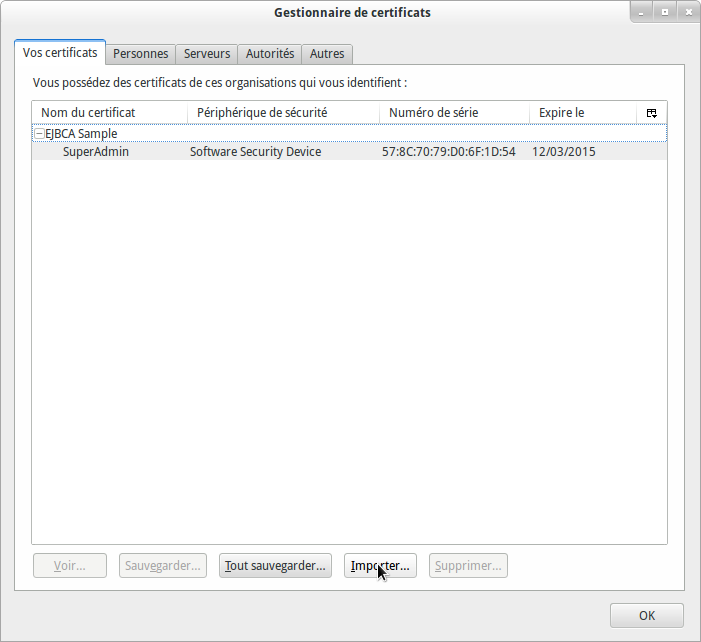
\includegraphics[width=30em]{import_superadmin.png}
\end{center}

On peut alors accéder à la partie administration à partir de l'adresse:

\verb+https://adresse_serveur:8443/ejbca/adminweb/index.jsp+
\newpage
La page obtenue est la suivante :
\begin{center}
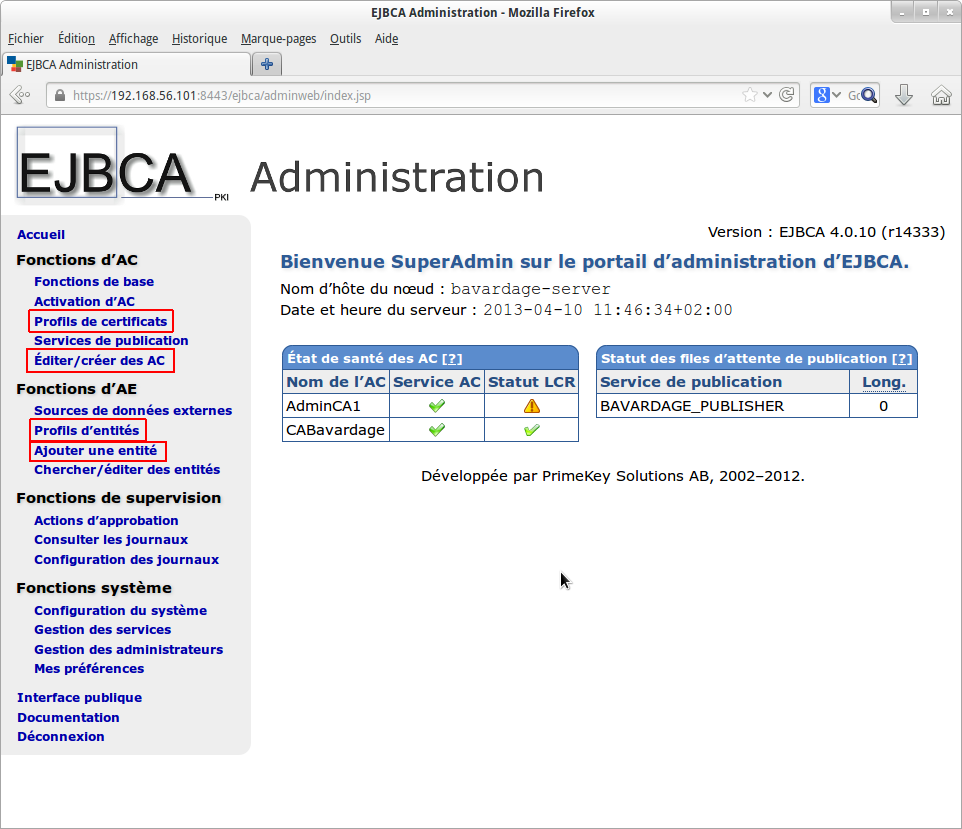
\includegraphics[width=40em]{admin_ejbca.png}
\end{center}

Les parties importantes ont été entourées en rouge et voici leurs descriptions.

\begin{paragraph}{Profils de certificats}
C'est dans cette section que l'ont créer les différents profils de certificats :
\begin{itemize}
\item \verb+BAVARDAGESERVER+ : profil pour le serveur sécurisé ;
\item \verb+BAVARDAGEUSER+ : profil pour les utilisateurs sécurisés.
\end{itemize}

Ces profils sont décrits en détail dans le document annexe : Politique de certification
\end{paragraph}

\begin{paragraph}{Éditer/créer des AC}
Une AC (autorité de certification) est une entité dont la mission est de vérifier les données du demandeur de certificat, de signer et de maintenir une liste des certificats et une liste des révocations. Sur la capture d'écran ci-dessus, on voit la liste des AC contenant celle relative à notre projet : \verb+CABavardage+
\end{paragraph}


\begin{paragraph}{Profils d'entités}
Chaque type d'entité a un profil associé:
\begin{itemize}
\item \verb+BAVARDAGE_SERVER+ : profil pour le serveur sécurisé ;
\item \verb+BAVARDAGE_USER+ : profil pour les utilisateurs sécurisés.
\end{itemize}
\end{paragraph}


\begin{paragraph}{Ajouter une entité}
Lorsqu'un utilisateur désire obtenir un certificat, un administrateur doit au préalable lui crée une entité associée. Il pourra ensuite récupérer son certificat pour sa clef RSA.
\end{paragraph}


\subsection{Partie sécurisée}
La troisième livraison consistait en la surcouche sécurisée du client de chat et d'un serveur « sécurisé » dont le rôle est de gérer les utilisateurs sécurisés.

Il a tout d'abord fallu ouvrir une connexion SSL entre le client sécurisé et le serveur sécurisé grâce aux fonctions d'OpenSSL. Ensuite, nous avons créer des codes d'actions spécifiques à l'utilisation sécurisée du chat comme \verb+CONNECT_SEC, CREATE_ROOM_SEC+... La gestion des clients dans le serveur sécurisé est similaire au serveur classique avec un fil d'exécution par client et une socket SSL.

Côté client, la surcouche sécurisée se base sur la librairie du client classique et utilise la même logique. Ainsi nous avons deux fonctions principales : 
\begin{itemize}
\item \verb+int send_message_sec (const char *mess, char **err_mess)+
\item \verb+int receive_message_sec (message *m)+
\end{itemize}

On rajoute également des fonctions de chiffrement/déchiffrement de messages :
\small{
\begin{itemize}
\item \verb+char *aes_encrypt (unsigned char *key, unsigned char *iv, char *plaintext, int *len)+
\item \verb+char *aes_decrypt (unsigned char *key, unsigned char *iv, char *ciphertext, int *len)+
\end{itemize}
}

Comme les noms des fonctions l'indiquent, nous utilisons AES-256-CBC pour chiffrer les messages envoyés (champ \verb+content+)


\section{Problèmes rencontrés}




\newpage
%%%%%%%%%%%%%%%%%%%%%%%%%%%%%%%%%%%%%%%%%%%%
% MANUEL D'UTILISATION 
% Charles & Ismaël
%%%%%%%%%%%%%%%%%%%%%%%%%%%%%%%%%%%%%%%%%%%%
\chapter{Manuel d'utilisation}
\section{Récupération du projet}
 Les sources du projet sont disponibles sur un dépôt git. Elles peuvent être récupérées en ligne de commande ou en ligne. 
 
 \subsection{En ligne de commande}
 Placez vous dans un terminal et exécutez la commande suivante :
\begin{verbatim} 
    $git clone git://github.com/legrajul/bavardage.git 
\end{verbatim}

\subsection{En ligne}
 Une archive contenant le projet peut être téléchargé à l'adresse :

\section{Compilation}
\subsection{Dépendances Ubuntu}
Pour la compilation du projet il faut d'abord vérifier si toutes les dépendances sont satisfaites :
\begin{itemize}
\item cmake : permet de compiler un projet pour différentes plateformes.
\item valac-0.18 : compilateur Vala qui traduit le code source vala en code source C.
\item libgtk-3-dev : outil multi plateformes pour créer des interfaces graphiques.
\item libgee-dev : librairies de collections fournissant des classes basées sur GObject.
\item libglib2.0-dev : fichiers de développement pour la bibliothèque GLib.
\item libssl-dev : bibliothèque de développement SSL.
\item libsqlite3-dev : bibliothèque de développement SQLite.

\end{itemize}

\subsection{Compilation des sources}

Les commandes suivantes doivent être exécuter dans le dossier du projet git bavardage : 
\begin{verbatim}
    $ mkdir src/build 
    $ cd src/build 
    $ cmake .. 
    $ make
\end{verbatim}

\section{Exécution}



\newpage
%%%%%%%%%%%%%%%%%%%%%%%%%%%%%%%%%%%%%%%%%%%%
% CONCLUSION 
% JB
%%%%%%%%%%%%%%%%%%%%%%%%%%%%%%%%%%%%%%%%%%%%


\newpage
\appendix
\chapter{Documents de gestion de projet}
\chapter{Déclaration des pratiques de certification}
\chapter{Politique de certification}
\end{document}